%\documentclass[draft]{beamer}
%\documentclass[handout]{beamer}
\documentclass{beamer}

% This file is a solution template for:

% - Giving a talk on some subject.
% - The talk is between 15min and 45min long.
% - Style is ornate.



% Copyright 2004 by Till Tantau <tantau@users.sourceforge.net>.
%
% In principle, this file can be redistributed and/or modified under
% the terms of the GNU Public License, version 2.
%
% However, this file is supposed to be a template to be modified
% for your own needs. For this reason, if you use this file as a
% template and not specifically distribute it as part of a another
% package/program, I grant the extra permission to freely copy and
% modify this file as you see fit and even to delete this copyright
% notice. 


\mode<presentation>
{
  \usetheme[compress]{Berlin}  
  %\usetheme{Berkeley}
  %\usecolortheme{sidebartab}
  % or ...
  \setbeamercovered{dynamic}
  % or whatever (possibly just delete it)
  \usefonttheme{professionalfonts}
  \setbeamertemplate{navigation symbols}{}
  \setbeamertemplate{footline}[frame number]
}


%****************************************************************************************************
% PACCHETTI
%****************************************************************************************************
% Tema principale
%\usetheme{Mainz}

%\usepackage{fontspec}
%\usepackage[libertine={Ligatures=TeX,RawFeature=+onum},biolinum={Ligatures=TeX,RawFeature=+onum}]{libertineotf}

\usepackage[biolinum,sfdefault]{libertine}
\usepackage{eulervm}

\usepackage[italian]{babel}

\usepackage[T1]{fontenc}
\usepackage[utf8]{inputenc}

%\usepackage{beamerfoils}
%\usepackage{array}
%\usepackage{mathrsfs}
\usepackage{booktabs}
\usepackage{color}
\usepackage{colortbl}    
\usepackage[version=3]{mhchem} 
%\usepackage{gensymb}
\usepackage{tabularx}
%\usepackage{cancel}
\usepackage[labelformat=empty,labelsep=none,skip=1pt]{caption}
\usepackage[per-mode=symbol]{siunitx}
\usepackage{relsize,xspace}
\usepackage{bm}
\usepackage{pgfpages}

\usepackage{tikz}
\usetikzlibrary{shapes,arrows,shadows,mindmap,trees,calc}

\usepackage{lipsum}

%****************************************************************************************************

%\setbeamercovered{dynamic}

\def\arrowd{
  (10.75:1.1) -- (6.5:1) arc (6.25:120:1) [rounded corners=0.5] --
  (120:0.9) [rounded corners=1] -- (130:1.1) [rounded corners=0.5] --
  (120:1.3) [sharp corners] -- (120:1.2) arc (120:5.25:1.2)
  [rounded corners=1] -- (10.75:1.1) -- (6.5:1) -- cycle
}

\tikzset{
  ashadow/.style={opacity=.25, shadow xshift=0.07, shadow yshift=-0.07},
}


%****************************************************************************************************
% COLORI e STILI di TESTO
\definecolor{greendark}{RGB}{0,178,140}
\definecolor{bluegreen}{cmyk}{0.9,0.0,0.35,0.2}
\definecolor{darkblue}{rgb}{0.2,0.2,0.65}
\definecolor{themecolor}{rgb}{0.137,0.466,0.741} % blue


%\newcommand{\cit}{\scriptsize\color{bluegreen}}             % citazioni
\newcommand{\cit}{\scriptsize\color{themecolor!80!green}}             % citazioni
\newcommand{\tbtit}{\bf\color{themecolor!75!black}} % titoli nelle tabelle
\newcommand{\ev}{\color{themecolor}\bf}
%\renewcommand{\CancelColor}{\color{red}}
%****************************************************************************************************


%****************************************************************************************************
% TABELLE
\newcolumntype{C}[1]{>{\centering\let\newline\\\arraybackslash\hspace{0pt}}m{#1}}
\setlength{\aboverulesep}{0pt}
\setlength{\belowrulesep}{0pt}
\setlength{\extrarowheight}{.75ex}
\arrayrulecolor{themecolor!75!black}

\newcommand{\tabitem}{~~\llap{\textbullet}~~}
%****************************************************************************************************


%****************************************************************************************************
% FRECCE
\tikzset{bluearrow/.style={draw=themecolor,fill=themecolor,single arrow,drop shadow=%
                           {shadow xshift=.3ex,shadow yshift=-.3ex,color=themecolor!60!black},
                           minimum height=3.5ex,minimum width=0.1ex,single arrow head extend=0.5ex,
                           single arrow tip angle=70}}

\newcommand{\arrowup}{\tikz[baseline=-0.5ex]{\node[bluearrow,rotate=90]{};}}
\newcommand{\arrowdown}{\tikz[baseline=-0.5ex]{\node[bluearrow,rotate=-90]{};}}
\newcommand{\arrowright}{\tikz[baseline=-0.5ex]{\node[bluearrow]{};}}
\newcommand{\arrowleft}{\tikz[baseline=-0.5ex]{\node[bluearrow,rotate=180]{};}}
%****************************************************************************************************


% COMANDI PERSONALI
\newcommand{\gete}{\ce{GeTe}\xspace}

% Path per le immagini
\graphicspath{{Immagini/}{../Thesis/Immagini/Plots/}{../THESIS/Immagini/}{../THESIS/Immagini/Plots/}{../THESIS/Immagini/bulk_figures/}}



%%% Layout di 4 pagine per foglio
%\pgfpagesuselayout{4 on 1}[a4paper,border shrink=5mm,landscape]


\title[] % (optional, use only with long paper titles)
{Simulazioni atomistiche del processo di cristallizzazione in nanofili di \gete}

%\subtitle
%{Molecular dynamics simulations in microcanonical ensemble} % (optional)

\author[] % (optional, use only with lots of authors)
{Edoardo Baldi\\\medskip {\small\emph{Relatore:} Prof.~Marco~Bernasconi}}
% - Use the \inst{?} command only if the authors have different
%   affiliation.
\institute[]{Università di Milano--Bicocca --- Dipartimento di Fisica}

\date[] % (optional)
{{\small Sessione di Laurea Magistrale del} \\[3pt] 23 marzo 2015}

%\subject{Molecular Dynamics}
% This is only inserted into the PDF information catalog. Can be left
% out. 

% If you have a file called "university-logo-filename.xxx", where xxx
% is a graphic format that can be processed by latex or pdflatex,
% resp., then you can add a logo as follows:

%\pgfdeclareimage[height=0.5cm]{university-logo}{Logo_Green}
%\logo{\pgfuseimage{university-logo}}


% If you wish to uncover everything in a step-wise fashion, uncomment
% the following command: 

%\beamerdefaultoverlayspecification{<+->}


\begin{document}

\begin{frame}
  \titlepage
\end{frame}

%\begin{frame}{Outline}
%  \tableofcontents
  % You might wish to add the option [pausesections]
%\end{frame}


\section{Introduzione}

\begin{frame}{Materiali a cambiamento di fase per memorie ottiche ed elettroniche}
\begin{minipage}{1.0\textwidth}
  \begin{minipage}[b]{0.53\linewidth}
  Memorie ottiche: {\ev DVD--RW,\\ Blu--ray Disc}
  \end{minipage}
\hfill
  \begin{minipage}[b]{0.43\linewidth}\centering
  \includegraphics[angle=0, width=0.4\textwidth]{DVD}
  \end{minipage}
\end{minipage}
\begin{minipage}{1.0\textwidth}
  \begin{minipage}[b]{0.53\linewidth}
  Memorie elettroniche non volatili:\hfill\\ {\ev memorie a cambiamento di fase} (PCM)
  \end{minipage}
\hfill
  \begin{minipage}[b]{0.43\linewidth}\centering
  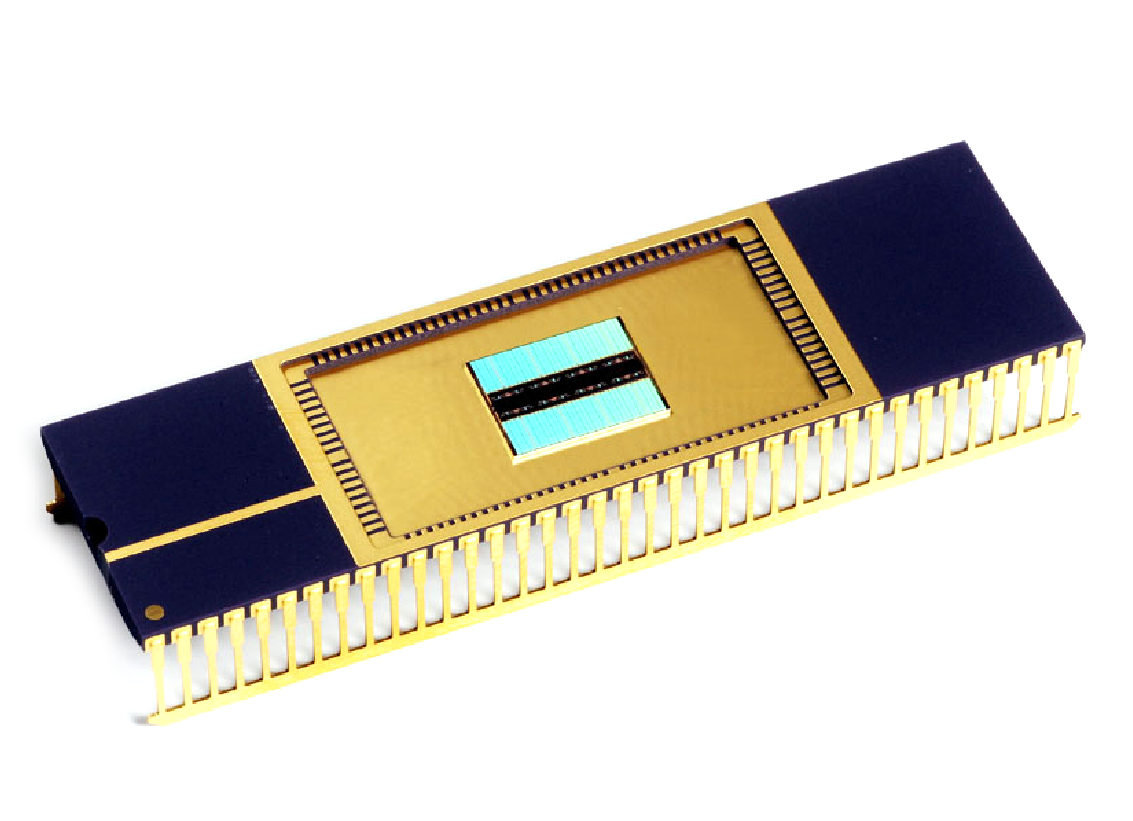
\includegraphics[angle=0, width=0.4\textwidth]{PCM}\\
  \end{minipage}
\end{minipage}
\vspace{1cm}\\
Leghe di calcogenuri: {\ev \gete}, \textcolor{themecolor}{\textbf{\ce{Ge2Sb2Te5} (GST)}}\\[6pt]
%\vspace{0.5cm}
\onslide<2->{
Rapida e reversibile transizione tra cristallo e amorfo ($\sim\SI{50}{ns}$)
}
\end{frame}


\begin{frame}{Materiali a cambiamento di fase}
\begin{table}
\begin{center}
\begin{tabular}{lcl}
Due stati della memoria & \arrowright & bit ``0'' o ``1''\\
\end{tabular}
\vspace{.5cm}\\
%\onslide<2->{
Grande differenza nelle proprietà tra le due fasi \\
%\vspace{1cm}
\begin{tabular}{ccc}
Fase cristallina & {\scriptsize $\arrowright$} & metallica \\
\end{tabular}
\quad
\begin{tabular}{ccc}
Fase amorfa & {\scriptsize $\arrowright$} & isolante\\
\end{tabular}
%}
\vspace{3ex}\\
%\onslide<3->{
\begin{tabular}{lcl}
Variazione di resistività di 3 ordini di grandezza & {\tiny $\arrowright$} & PCM\\
Differenza della riflettività del 30\% & {\tiny $\arrowright$} & memorie ottiche\\
\end{tabular}
\vspace{0.5cm}\\
La transizione è indotta per riscaldamento (impulsi laser/corrente)
%}
\end{center}
\end{table}
\end{frame}


\begin{frame}{Cella PCM}
\begin{columns}
 \begin{column}{0.5\textwidth}
  \begin{itemize}
   \item {\ev Regione attiva}: piccola porzione del film di materiale che subisce la transizione
   \item Transizione indotta per effetto Joule
  \end{itemize}
 \end{column}
 \begin{column}{0.5\textwidth}
   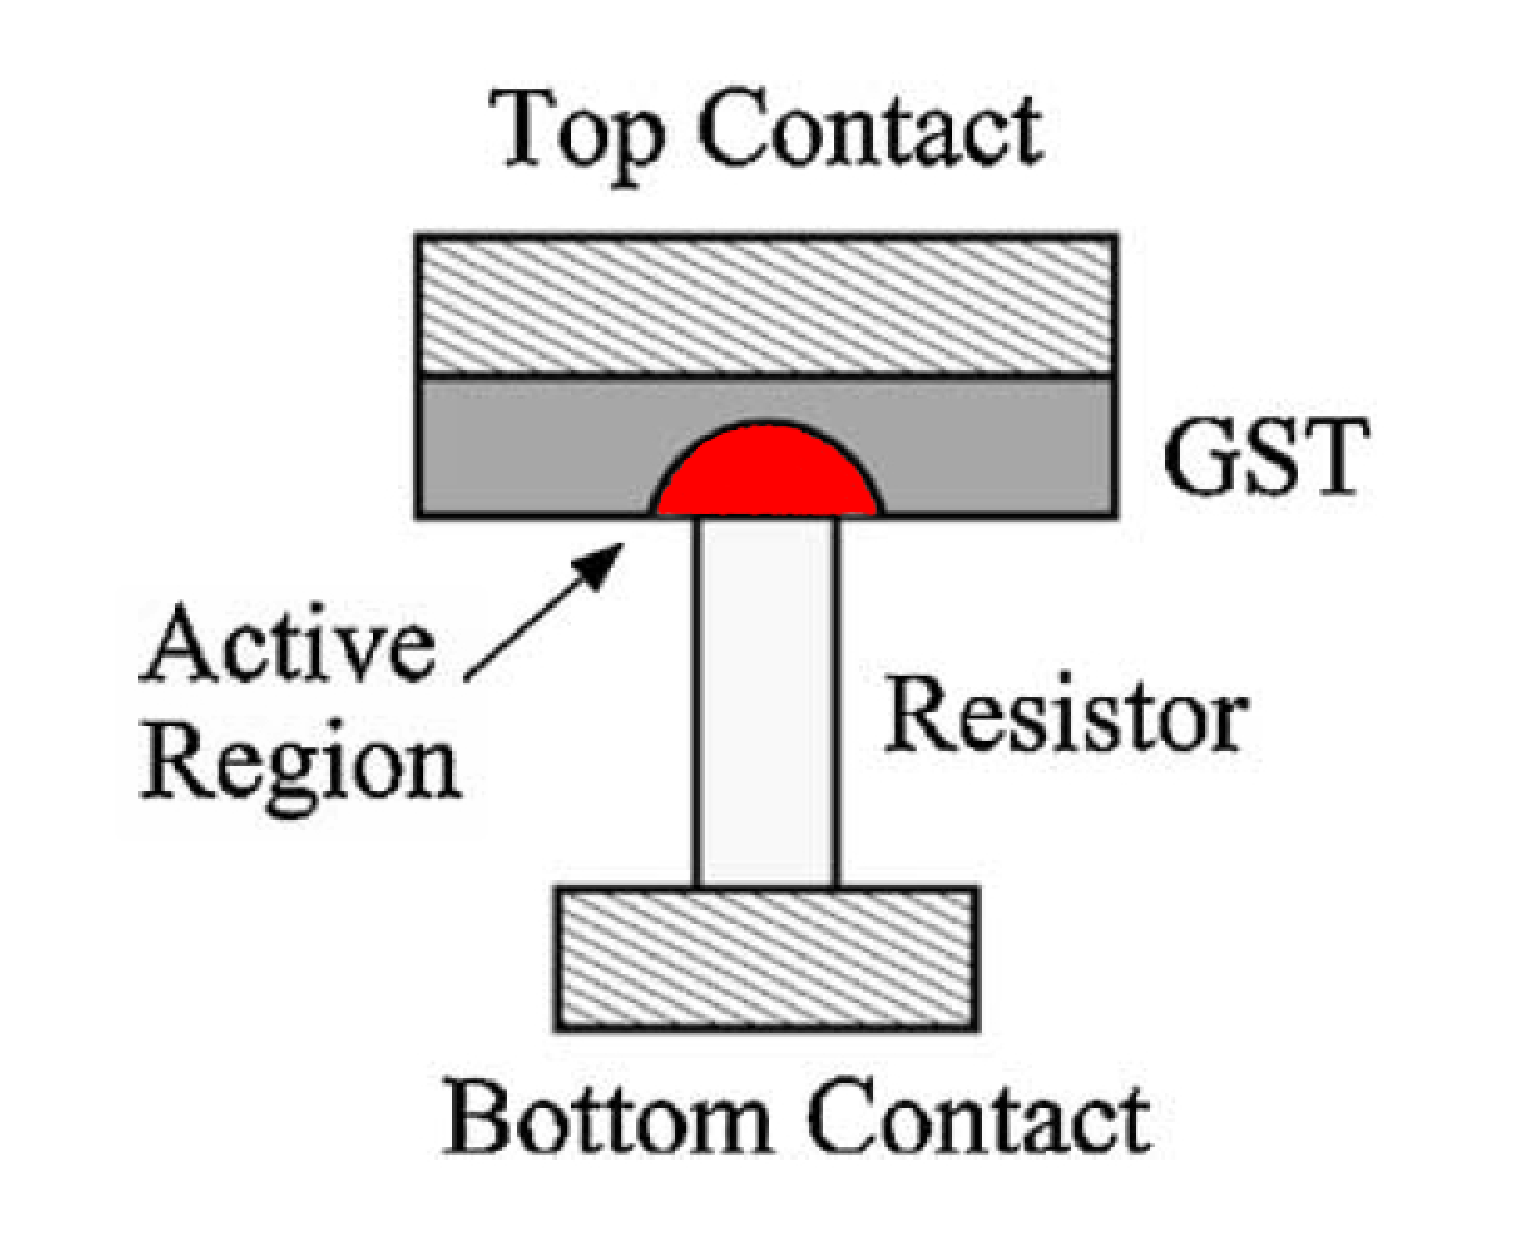
\includegraphics[scale=0.2]{PCMschem}
  %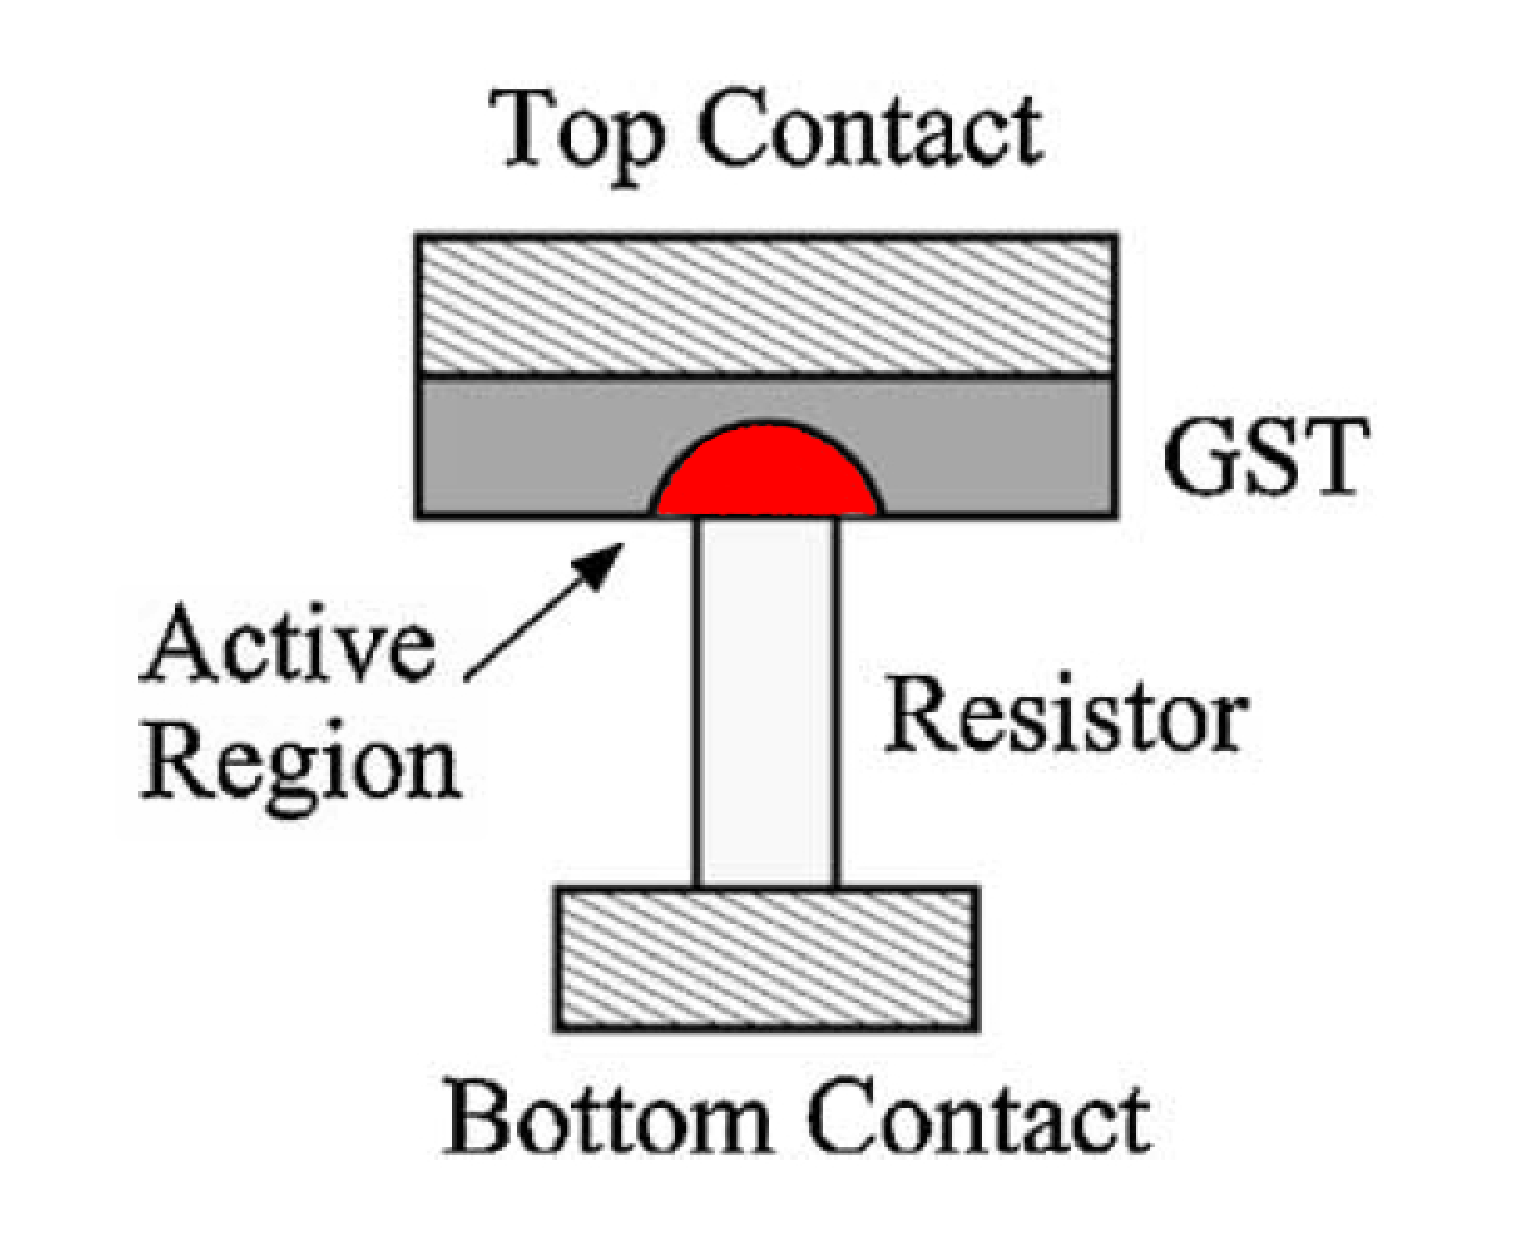
\includegraphics[width=0.5\textwidth]{PCMschem}
 \end{column}
\end{columns}
\end{frame}

%\begin{minipage}[c]{0.58\linewidth}
%\begin{flushright}
%\end{flushright}
%\end{minipage}
%\vspace{-0.05\textheight}
%\begin{minipage}[c]{0.38\linewidth}
%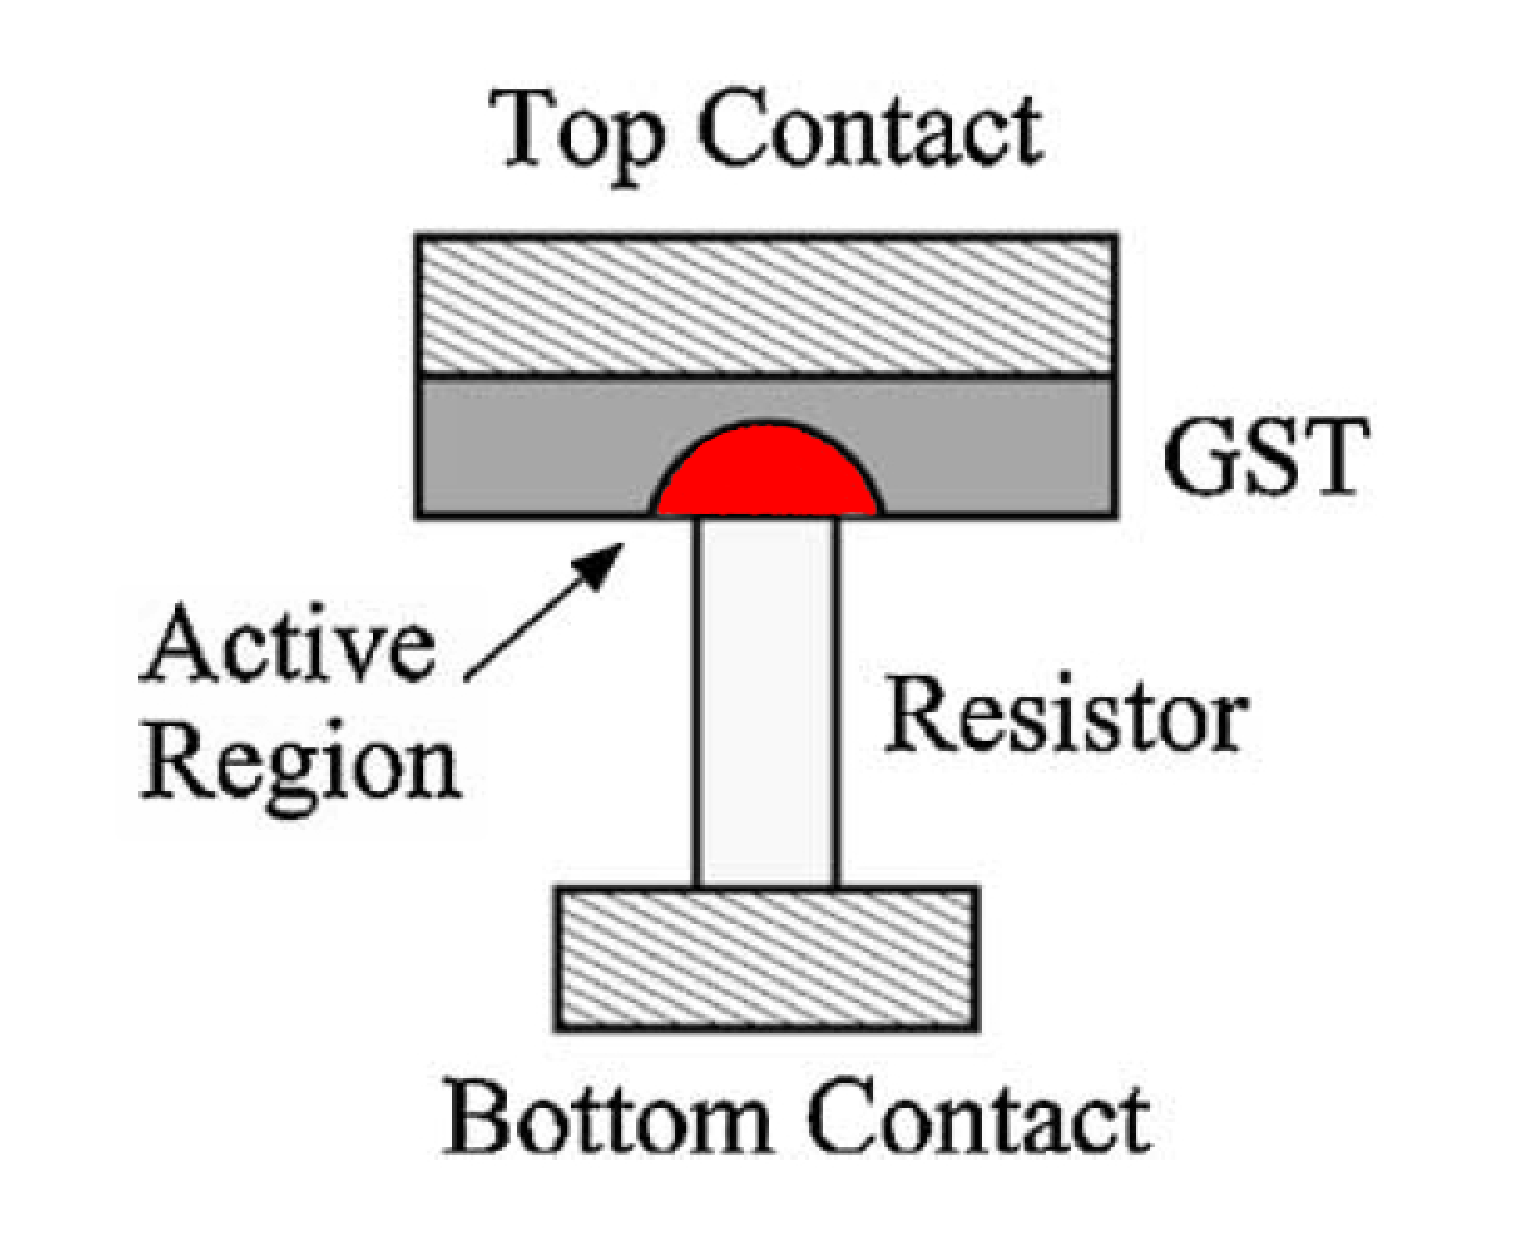
\includegraphics[angle=0, width=0.9\textwidth]{PCMschem.eps}\\
%\end{minipage}
%\begin{minipage}[c]{0.48\linewidth}
%\centering
%\includegraphics[angle=0, width=0.9\textwidth]{PCM_SEM.eps}
%\end{minipage}
%\vspace{2ex}
%\begin{minipage}[c]{0.48\linewidth}
%\small{
%\begin{itemize}
%\item Active region: a small drop within GST film undergoes the phase transition\\
%\item Phase-change by heating via Joule effect
%\end{itemize}
%\begin{center}
%Concept first proposed by\\
%Ovshinsky in 1968
%\end{center}
%}
%\end{minipage}

\begin{frame}{Caratteristica I--V di una cella PCM}
\begin{columns}
 \begin{column}{0.5\textwidth}
  \begin{itemize}
    \item<2> \emph{Lettura}: eseguita a bassa tensione ($V < V\ped{th}$)
    \item<3-> Processi di \emph{set/reset}: tensione applicata maggiore del valore $V\ped{th}$)
    \begin{itemize}
      \item<3-> \emph{Reset}: elevata intensità di corrente e impulso breve \\
		\ev{cristallo} $\rightarrow$ \ev{amorfo}
      \item<4-> \emph{Set}: bassa intensità e impulso più lungo \\
		\ev{amorfo} $\rightarrow$ \ev{cristallo}
    \end{itemize}
   \end{itemize}
 \end{column}
  \begin{column}{0.5\textwidth}
   \includegraphics<1>[angle=0, width=1.0\textwidth]{IV1}
   \includegraphics<2>[angle=0, width=1.0\textwidth]{IVr}
   \includegraphics<3>[angle=0, width=1.0\textwidth]{IVres}
   \includegraphics<4>[angle=0, width=1.0\textwidth]{IVs}
  \end{column}
\end{columns}
\end{frame}

\begin{frame}
\frametitle{PCM commerciali}
{\ev Aprile 2010} 
\hspace{10em}\raisebox{-1ex}{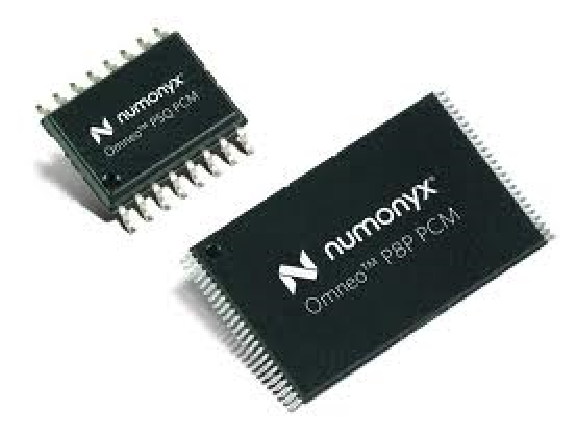
\includegraphics[angle=0, width=0.2\textwidth]{PCM_numonyx.eps}}\\
\vspace{1ex}
\textcolor{themecolor}{Numonyx} (ora \textcolor{themecolor}{Micron}) ha commercializzato un dispositivo PCM di 90~nm\\
%Research center based in Agrate Brianza\\
\vspace{3ex}
{\ev Luglio 2012}\\
\vspace{1ex}
\textcolor{themecolor}{Numonyx}: dispositivo a 45~nm\\ %(Agrate)\\
%\vspace{1ex}
\begin{columns}[c]
\column{0.00\textwidth}
\column{0.70\textwidth}
{\ev Gennaio 2013}\\
\vspace{1ex}
\textcolor{themecolor}{Nokia}: telefono cellulare ``Asha'' con\\
dispositivo PCM Micron %(NOR replacement)\\
\column{0.30\textwidth}
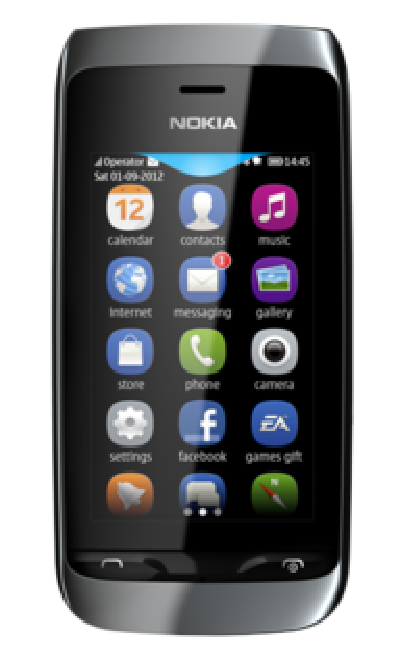
\includegraphics[angle=0, width=0.4\textwidth]{nokia.eps}
\end{columns}
\end{frame}


\begin{frame}{Nanofili nei dispositivi PCM}
 \begin{exampleblock}{Vantaggi nell'utilizzo di nanofili}
  \begin{itemize}
   \item Riduzione delle dimensioni della cella
   \item Riduzione della potenza dissipata nel processo di programmazione
   \item Effetti di confinamento del calore
  \end{itemize}
\end{exampleblock}
\note<1>{%
  Sono state proposte diverse architetture per ridurre la potenza dissipata nel processo di programmazione. Una di queste consiste nel sostituire al film di materiale attivo, un nanofilo, che permette un miglior confinamento del calore e in principio consente anche una riduzione delle dimensioni della cella.
}
\end{frame}


\begin{frame}{La cristallizzazione}
%\only<1>
%\only<2>{%
% \begin{alertblock}{}
% La cinetica di cristallizzazione è di difficile approccio sperimentale\\[3pt]
% \end{alertblock}
%}
\only<1>{%
 \centering
 {\ev Teoria della nucleazione e crescita}\\[0.5cm]
 \begin{columns}
  \begin{column}{0.5\textwidth}
   \centering
   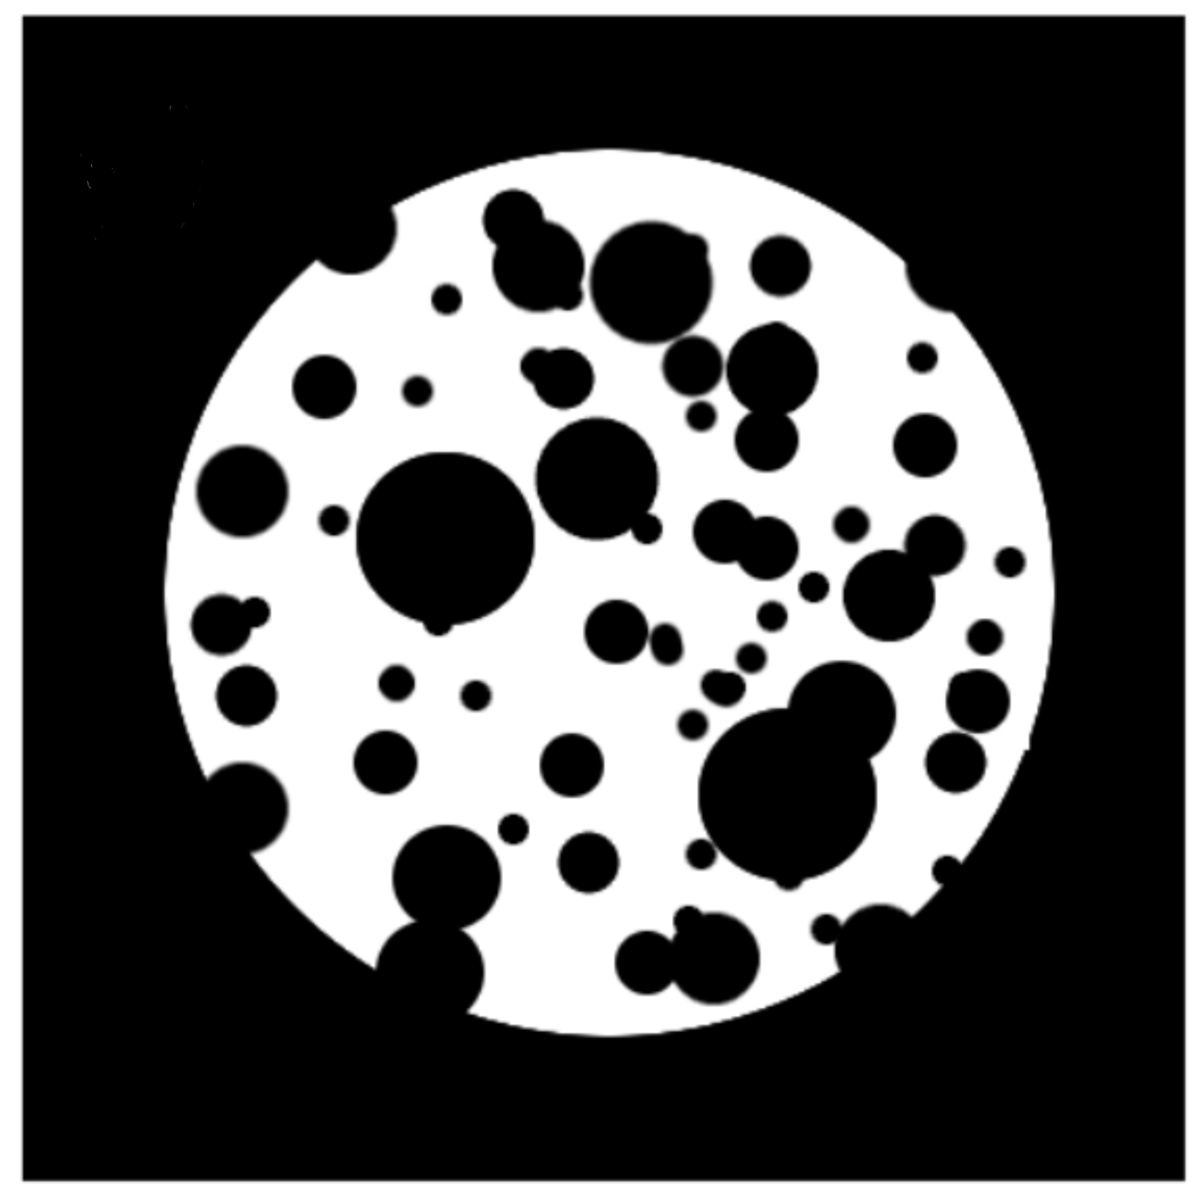
\includegraphics[width=0.3\textwidth]{N-dominated}\\[6pt]
   {\ev \emph{Nucleation--driven}}
  \end{column}
  \begin{column}{0.5\textwidth}
   \centering
   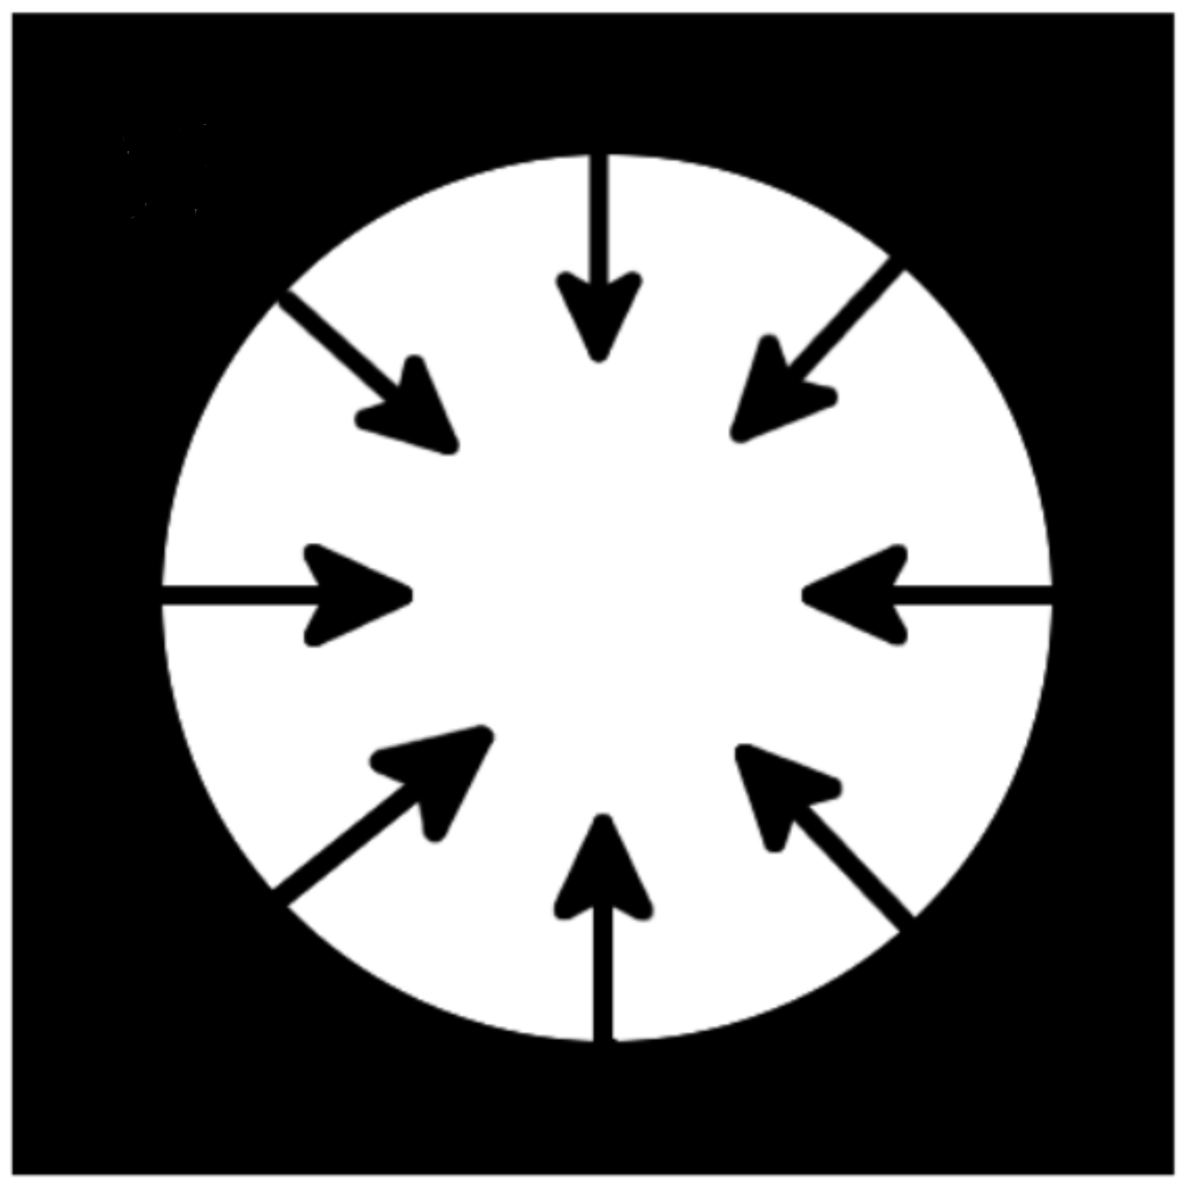
\includegraphics[width=0.3\textwidth]{G-dominated}\\[6pt]
   {\ev \emph{Growth--driven}}
  \end{column}
 \end{columns}
 %\begin{alertblock}{}
 % La cinetica di cristallizzazione è di difficile approccio sperimentale 
 %\end{alertblock}
}
%\vspace{.1cm}
\only<2>{%
  \begin{itemize}
   \item Il meccanismo di cristallizzazione dipende dalla dimensione della fase amorfa, dalla temperatura e dal materiale
   \item Nelle PCM la fase amorfa è portata a $T$ molto maggiori di $T\ped{glass}$ (liquido sotto--raffreddato)
   \item La cinetica di cristallizzazione può cambiare da \emph{bulk} a nanofili \\[3pt]
      $T\ped{fus}$ e $T\ped{glass}$ dipendono dalle dimensioni
  \end{itemize}

}
\end{frame}



\section{Nanofili di \gete}

\begin{frame}{\gete: struttura cristallina}
 \begin{columns}
  \begin{column}{0.4\textwidth}
      \begin{itemize}
       \item<1-> Struttura cristallina {\ev trigonale} (fase $\alpha$) con cella elementare {\ev romboedrica}
       \item<1-> Struttura cubica tipo \ce{NaCl} elongata lungo la $\langle 111 \rangle$
       \item<2-> Parametri strutturali
      %\onslide<3->{% 
       %\begin{itemize}
        %\item 
        $a=\SI{4.31}{\angstrom}$\\
        %\item 
        $\alpha=\ang{57.9}$\\
        %\item 
        $x=\num{0.2366}$ \\[3pt] Ge: $(x,\,x,\,x)$ \\[3pt] Te: $(-x,\,-x,\,-x)$
       %\end{itemize}
       %}
       \note<2>{%
	 I parametri strutturali della struttura trigonale sono il passo reticolare $a$, l'angolo tra una coppia di vettori di base $\alpha$ e il parametro $x$ che assegna le posizioni nella cella elementare dei due atomi di Ge e Te. 
	}
      \end{itemize}
  \end{column}
  \begin{column}{0.4\textwidth}
   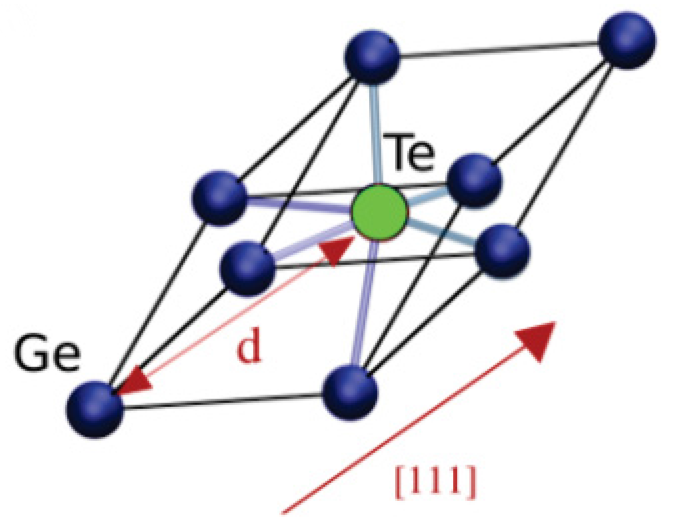
\includegraphics[width=0.7\textwidth]{GeTe-cell}\\[12pt]
   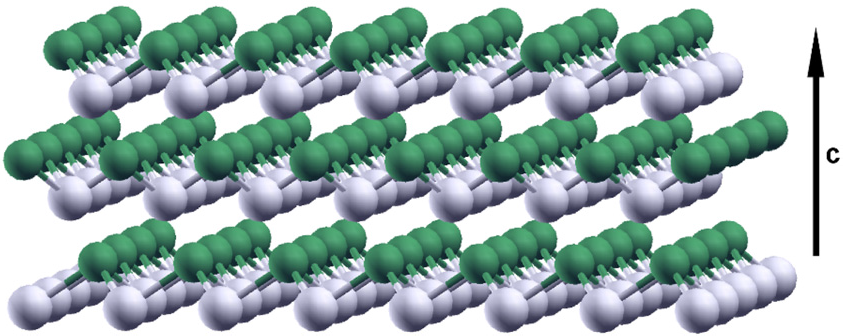
\includegraphics[width=\textwidth]{GeTe-bilayer}
  \end{column}

 \end{columns}

\end{frame}

\begin{frame}{Nanofilo: il modello}
 \begin{columns}
  \begin{column}{0.5\textwidth}
    \begin{itemize}
      \item Nanofilo cresciuto lungo la {\ev direzione $[110]$}\\ (notazione esagonale)
      \item Diametro di $\sim \SI{8}{nm}$
      \item Supercella di simulazione \\ {\ev$l=\SI{84.65}{\angstrom}$} e {\ev\num{16540} atomi}
      \item PBC lungo l'asse di crescita
  \end{itemize}
  \end{column}
  \begin{column}{0.5\textwidth}
   \centering
   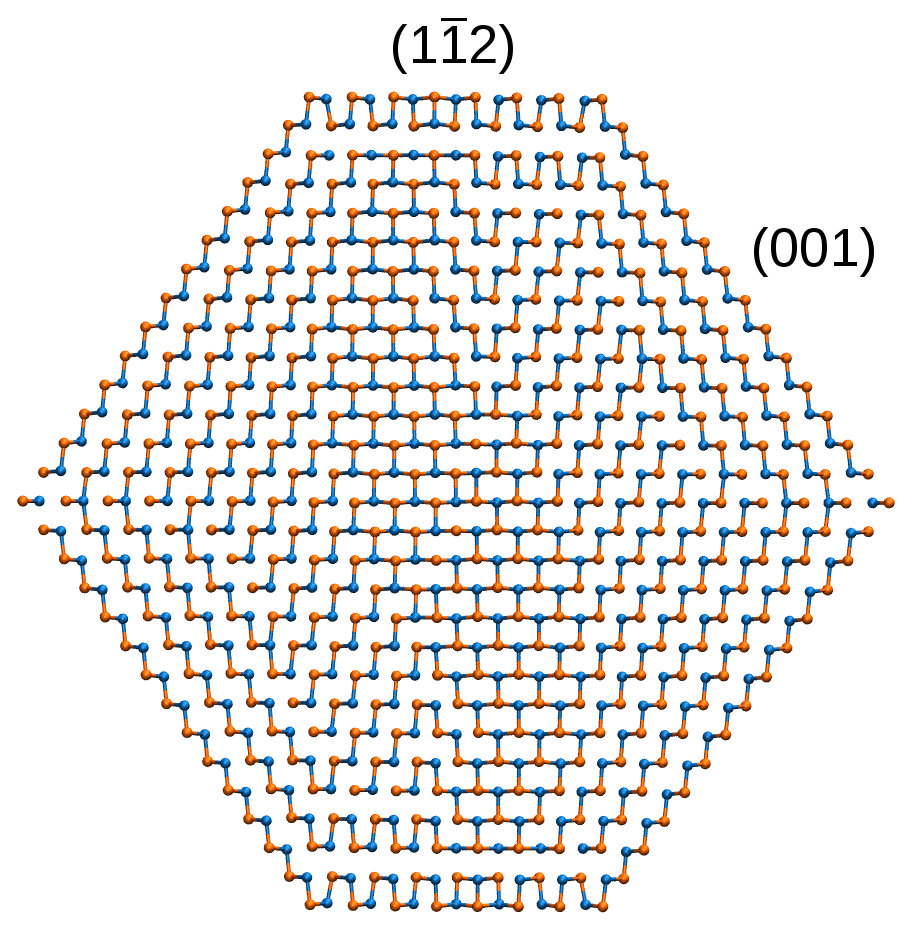
\includegraphics[width=0.35\textheight]{nw_section_OK}\\[3pt]
   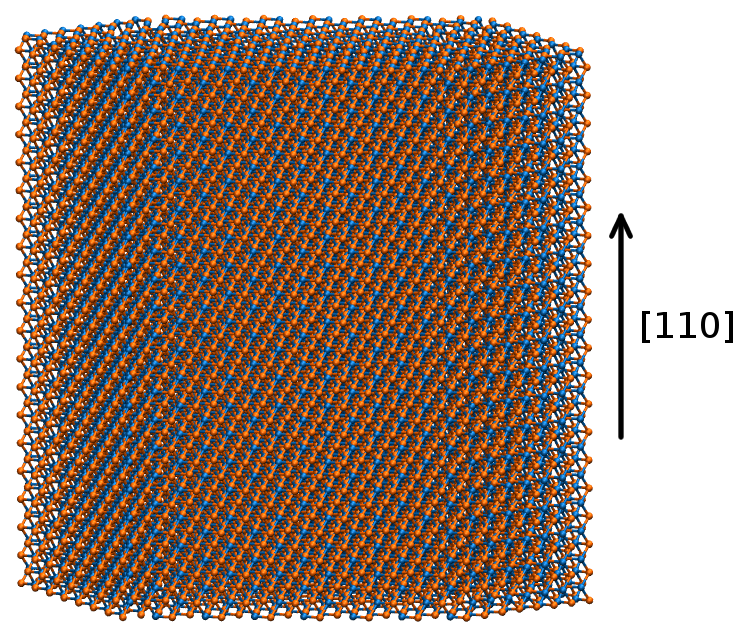
\includegraphics[width=0.35\textheight]{nw_long_OK_wDir}
  \end{column}
 \end{columns}
 \vspace{0.2cm}
 \centering
 Simulazioni di {\ev dinamica molecolare} del processo di cristallizzazione con potenziale interatomico
\end{frame}





\section{Metodi computazionali}
%\subsection{Potenziale \emph{neural networks}}
%\begin{frame}{Dinamica molecolare con potenziale \emph{neural networks}}
% MD e potenziale NN
%\end{frame}

%\subsection{Potenziale NN}

\begin{frame}{Potenziale \emph{neural networks}}
 \centering
Energia totale come somma di energie atomiche: $E_{tot} = \sum_i E_i$
\note<1>{%
The neural network potential is built by writing the total energy as 
a sum of the atomic energies which depend on the atomic local environment. 
And the local environment is described by the symmetry functions $G$ 
which depend on bond lengths and bond angles up to a certain cut-off distance 
that in our case include the third coordination shell.\\
The neural network is a scheme to assign an energy to a single atom given the 
local environment. The atomic energy is an analytic function of the atomic 
positions, so it is easy to calculate forces. 
}
\begin{flushright}
{\cit{[J.~Behler e M.~Parrinello, PRL 98, 146401 (2007)]}}
\end{flushright}
%
%\vspace{3ex}
\onslide<2->{%
  \begin{columns}[c]
    \begin{column}{0.50\textwidth}
      \begin{equation*}
	E_i = F(\{G(\vec{x})\}) 
      \end{equation*}
      \vspace{.5cm}
      \centering
      \resizebox*{0.8\textwidth}{!}{%%% TiKz picture of NN scheme
\begin{tikzpicture}
  %%Create a style for the arrows we are using
  \tikzset{normal arrow/.style={draw,-stealth',very thick,color=themecolor}}
  \tikzset{little arrow/.style={draw,-stealth',thick,color=themecolor!60!white}}
  \tikzset{node circle/.style={circle,shading=ball,ball color=themecolor,text=white}}
  \tikzstyle{layer} = [text width=4em, text centered]
  %%Create the different coordinates to place the nodes
  \path (0,0) coordinate (g1) ++(0,-2.5) coordinate (g2); %++(0,-2) coordinate (3);
  \path (g1) ++(-1.3,-.5) coordinate (x1);
  \path (g2) ++(-1.3,+.5) coordinate (x2);
  %%Use the calc library and partway modifiers to generate the second and third level points
  \path ($(g1)!.5!(g2)!2.2 cm!90:(g2)$) coordinate (y2);
  \path (y2) ++(0,2) coordinate (y1);
  \path (y2) ++(0,-2) coordinate (y3);
  \path (y2) ++(1.7,0) coordinate (e);
  %%Place nodes at each point using the foreach construct
  \foreach \in/\i/\color in {g1/1/themecolor!60,g2/2/themecolor!60}{
%    \node[draw,circle,shading=axis,top color=\color, bottom color=\color!black,text=white,shading angle=45] (n\in) at (\in) {$G_{\i}$};
    \node[node circle] (n\in) at (\in) {$G_{\i}$};
  }
  \foreach \in/\i/\color in {y1/1/themecolor!60,y2/2/themecolor!60,y3/3/themecolor!60}{
%    \node[draw,circle,shading=axis,top color=\color, bottom color=\color!black,text=white,shading angle=45] (n\in) at (\in) {$y_{\i}$} 
%         node[above of =n\in,node distance=2em]{$f_{\i}$};
    \node[node circle] (n\in) at (\in) {$y_{\i}$} node[above of =n\in,node distance=2em]{$f_{\i}$};
  }
%  \node[draw,circle,shading=axis,top color=themecolor!60, bottom color=themecolor!60!black,text=white,shading angle=45] (ne) at (e) {$\;\;E_{i}\;\;$}; 
  \node[node circle] (ne) at (e) {$\;\;E_{i}\;\;$};
  %%Place the remaining nodes separately
  \node (nx1) at (x1) {$\bm{x}_1$};
  \node (nx2) at (x2) {$\bm{x}_2$};
  %%Layer titles
  \node[layer,above of=ny2, node distance=22ex] (hl) {Hidden layer};
  \node[layer,left of=hl, node distance=2.2cm] (il) {Input layer};
  \node[layer,above of=e, node distance=22ex] (ol) {Output layer};
  %%Drawing the arrows
  \path[little arrow] (nx1) -- (ng1);
  \path[little arrow] (nx1) -- (ng2);
  \path[little arrow] (nx2) -- (ng1);
  \path[little arrow] (nx2) -- (ng2);
  \path[normal arrow] (ng1) -- node[above=.0em] {$a_{11}^{01}$} (ny1);
  \path[normal arrow] (ng1) -- node[above=.0em] {$a_{12}^{01}$} (ny2);
  \path[normal arrow] (ng1) -- node[below=-2.0em,left=1.4em] {$a_{13}^{01}$} (ny3);
  \path[normal arrow] (ng2) -- (ny1);
  \path[normal arrow] (ng2) -- (ny2);
  \path[normal arrow] (ng2) -- node[below=0.0em] {$a_{23}^{01}$} (ny3);
  \path[normal arrow] (ny1) -- node[above=0.2em] {$a_{11}^{12}$} (ne);
  \path[normal arrow] (ny2) -- node[above=0.1em] {$a_{21}^{12}$} (ne);
  \path[normal arrow] (ny3) -- node[above=0.5em] {$a_{31}^{12}$} (ne);
\end{tikzpicture}}
    \end{column}
\note<2>{%
This picture represent a simple scheme of a neural network.
The symmetry functions are obtained from the atomic positions and are the input 
values of the network. We take a linear combination of the symmetry functions with 
these weights $a$ to obtain these intermediate values $y$. Then we apply a non linear 
function $f$ with this form to the $y$s and the results are again linearly combined to 
obtain the atomic energy. The weights $a$ are the fitting parameters of the potential. 
In our case for GeTe the network has 8 thousand parameters fitted on 30 thousand 
configurations.  
}
%
\begin{column}{0.50\textwidth}
\centering
{\ev{Symmetry function $\{G\}$}}\\
Informazioni sull'intorno atomico entro un certo raggio di \emph{cutoff} (terza \emph{shell} di coordinazione)\\[12pt]}
\onslide<3->{%
  $E_i$ è funzione analitica delle posizioni degli atomi
  \begin{equation*}
    E_i = \sum_{j=1}^3{a_{j1}^{12}\cdot f\left(\sum_{k=1}^2{G_k\cdot a_{kj}^{01}}\right)}
  \end{equation*}

}
\end{column}
\end{columns}
\end{frame}


%\subsection{Potenziale NN per il \gete}
\begin{frame}{Potenziale \emph{neural networks} per il \gete}
\only<1>{%
  \begin{itemize}
    \item $E_i$ è calcolata con il metodo \emph{neural networks}
    \item Il potenziale per il \gete è ottenuto interpolando un database di energie calcolate \emph{ab initio}
    \item \num{30000} configurazioni e $\sim\num{8000}$ parametri
  \end{itemize}
}
%
\only<2>{%
 \begin{columns}
  \begin{column}{0.5\textwidth}
  \centering
  {\footnotesize\textcolor{themecolor}{Funzioni di correlazione di coppia per \gete amorfo a \SI{300}{K}}}\\
   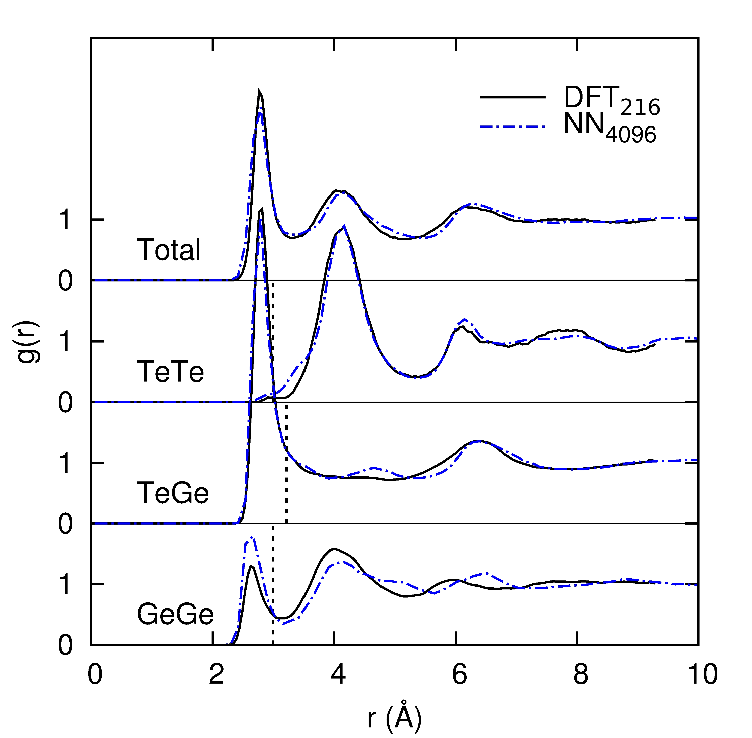
\includegraphics[width=\textwidth]{GT_grNN_DFT}\\
   %{\Large\slshape FIGURA}\\[0.2cm]   
   {\cit{[Sosso et al., PRB 85, 174103 (2012)]}}
  \end{column}
  \begin{column}{0.5\textwidth}
   \begin{itemize}
    \item Il potenziale NN descrive accuratamente le proprietà della fase liquida/amorfa del \gete
    \item Coefficiente di diffusione $D$: {\ev \SI{4.29e-5}{\square\centi\metre\per\second}}\\ (DFT~\SI{4.29e-5}{\square\centi\metre\per\second})
    \item $T\ped{fus}$: {\ev\SI{1001}{K}}\\ (exp.~\SI{998}{K})
   \end{itemize}
  \end{column}
 \end{columns}
 }
\end{frame}




\section{Risultati}

\begin{frame}{Cristallizzazione in \emph{bulk}}
\only<1>{%
\centering
Interfaccia tra cristallo e liquido sotto--raffreddato
  \begin{columns}
  \begin{column}{0.5\textwidth}
   \begin{itemize}
    \item Simulazioni $NVT$ per $\sim \SI{100}{ps}$
    \item Atomi cristallini identificati secondo il parametro d'ordine
      \[ \mathsmaller{q_{4m}(i) = \frac{1}{N_b (i)} \sum_{j=1}^{N_b(i)} Y_{4m}(\bm{r}_{ij})} \]
      \begin{flushleft}
       {\cit{[Steinhardt et al., PRB 28, 784 (1983)]}}
      \end{flushleft}
    \item Spessore dello \emph{slab} cristallino L\ped{cris} in funzione di t
   \end{itemize}
  \end{column}
%
  \begin{column}{0.5\textwidth}
  \centering
   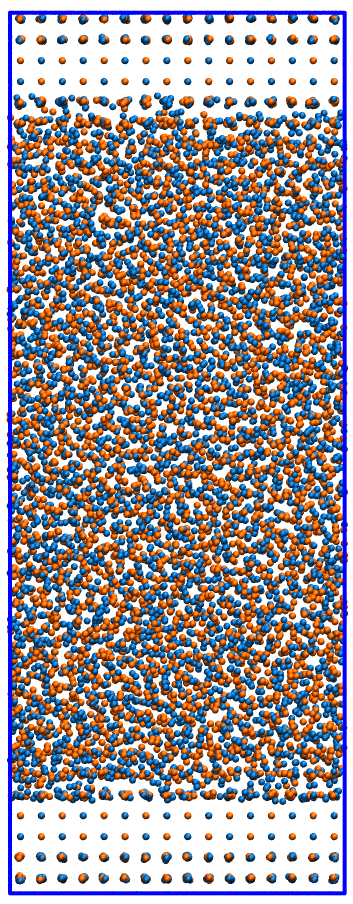
\includegraphics[scale=0.15]{m1_long_OK}\quad
   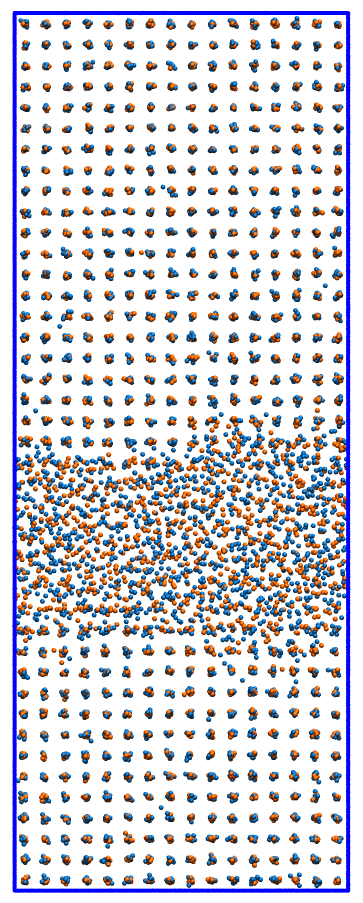
\includegraphics[scale=0.15]{m1_AfterCry}
  \end{column}
 \end{columns}
}
\only<2>{%
  \begin{columns}
   \begin{column}{0.5\textwidth}
    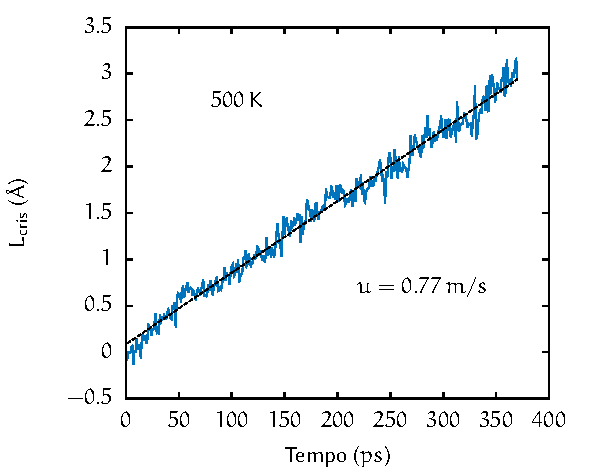
\includegraphics[width=\textwidth]{bulk_Lcr_500_OK}
   \end{column}
   \begin{column}{0.5\textwidth}
    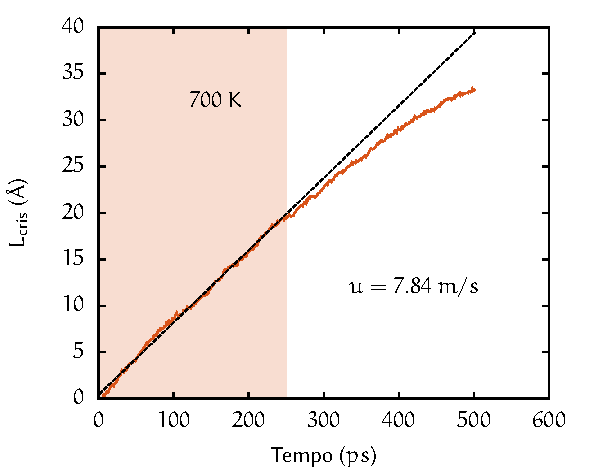
\includegraphics[width=\textwidth]{bulk_Lcr_700_OK}
   \end{column}
  \end{columns}
 \vspace{.5cm}
 \centering
 Velocità di crescita
 \[ u = \frac{dL\ped{cris}}{dt} \]
}
\end{frame}

\begin{frame}{Temperatura di fusione}
%\centering
Stima della temperatura di fusione nei nanofili\\[12pt]
\begin{columns}
\begin{column}{0.4\textwidth}
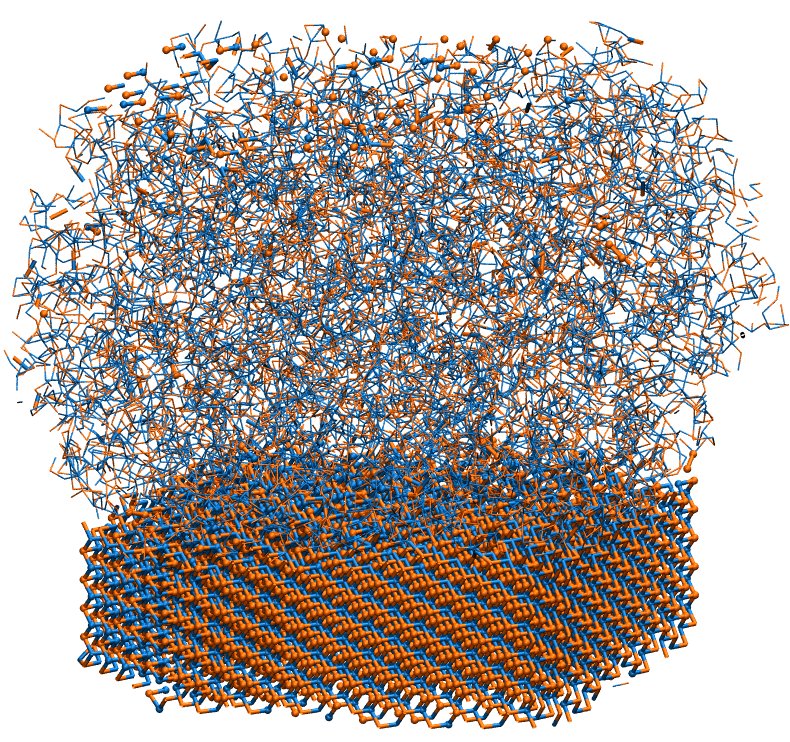
\includegraphics[width=\textwidth]{nw_superc}
\end{column}
%
\begin{column}{0.6\textwidth}
%\begin{itemize}
%\item
 4 simulazioni $NVT$ a \num{800}--\num{850}--\num{900}--\SI{950}{K}:\\[3pt]
  \begin{itemize}
    \item a \SI{800}{K} {\ev cristallizzazione}
    \item a \SI{850}{K} {\ev fusione}
  \end{itemize}
%\end{itemize}
\end{column}
\end{columns}
\onslide<2->{%
\begin{exampleblock}{Riduzione di T\ped{fus}}
\centering
  $\SI{800}{K} < T\ped{fus}^N < \SI{850}{K}$\\[6pt]
  $T\ped{fus}^B \sim \SI{1000}{K}$
\end{exampleblock}
}

\end{frame}



%\subsection{Generazione del liquido}

\begin{frame}{Generazione del liquido \emph{supercooled}}
 \begin{columns}
  \begin{column}{0.5\textwidth}
   \begin{itemize}
    \item Generato portando una parte del nanofilo a $T > T_m$ in \SI{30}{ps}
    \item Equilibrato per \SI{10}{ps} in $NVE$
    \item Raffreddato rapidamente (\SI{30}{ps}) a \num{700}--\num{600}--\SI{500}{K}
   \end{itemize}

  \end{column}
  \begin{column}{0.5\textwidth}
   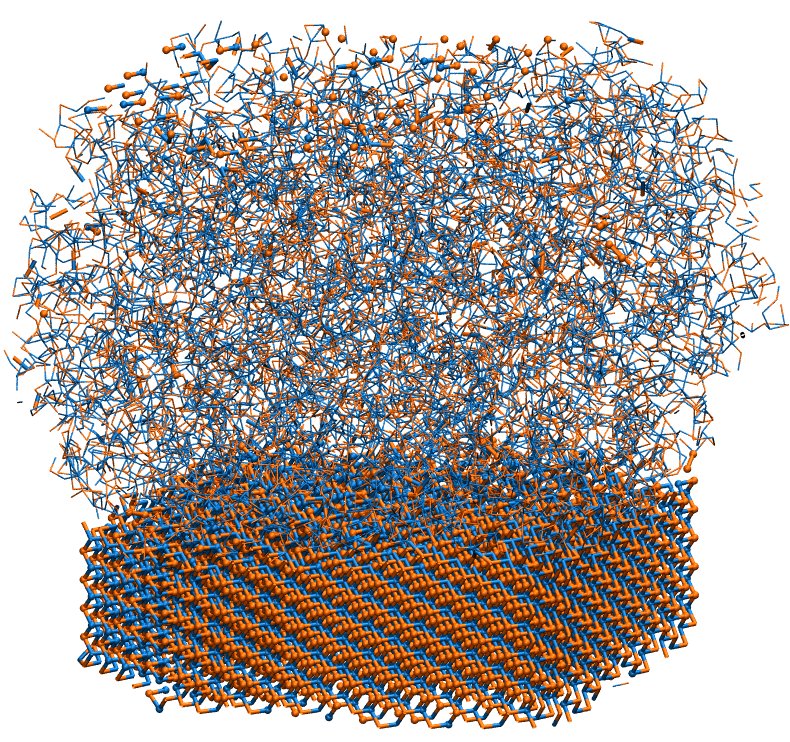
\includegraphics[width=\textwidth]{nw_superc}
  \end{column}
 \end{columns}
\end{frame}


\begin{frame}{Cristallizzazione nel nanofilo}
  \begin{columns}
   \begin{column}{0.5\textwidth}
    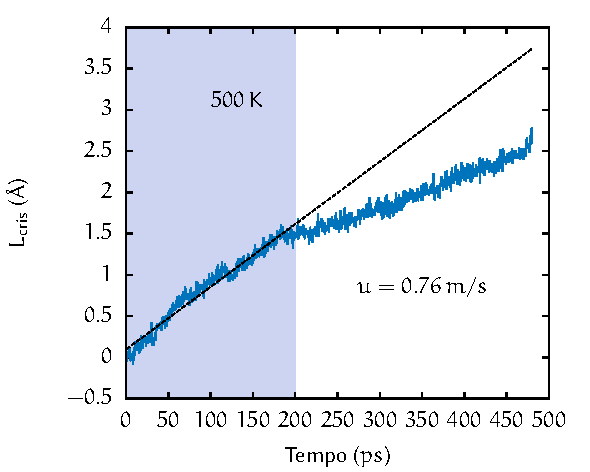
\includegraphics[width=\textwidth]{nw_Lcr_500_OK}
   \end{column}
   \begin{column}{0.5\textwidth}
    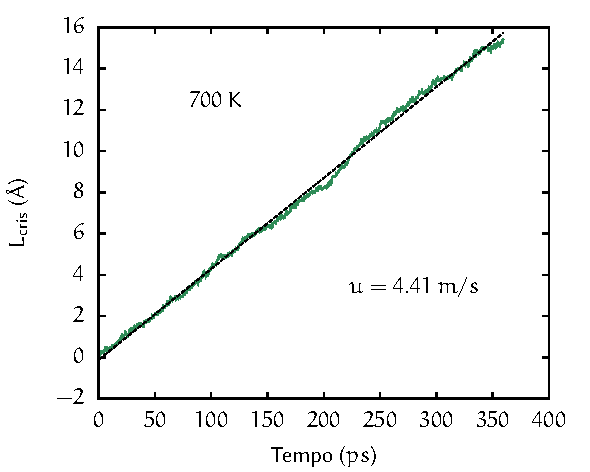
\includegraphics[width=\textwidth]{nw_Lcr_700_OK}
   \end{column}
  \end{columns}
  \begin{table}[h]
   \resizebox*{0.3\textwidth}{!}{%
    \begin{tabular}{cSS}
     	\toprule
     	\rowcolor{themecolor!20!white}
	T (\si{K}) & \multicolumn{2}{S}{ {u (\si{\metre\per\second})} } \\
	\cmidrule{2-3}
		& {\small Nanofilo} & {\small Bulk} \\
	\midrule
	\num{500} & 0.76 & 0.77 \\
	\num{700} & 4.41 & 7.84 \\
	\bottomrule
    \end{tabular}}
  \end{table}

\end{frame}




\begin{frame}{Velocità di cristallizzazione}
 Velocità di crescita secondo la \emph{teoria classica della nucleazione}
 %\centering
  \begin{equation*}
    u(T)= \frac{6D}{\lambda} \left[ 1- e^{ \left( -\Delta\mu/k_B T\right) } \right]
  \end{equation*}
  \begin{center}
  \begin{itemize}
   \item $D$ = coefficiente di auto--diffusione
   \item $\lambda$ = distanza interatomica media ($\sim \SI{3}{\angstrom}$)
   \item $\Delta\mu$ = differenza di potenziale chimico tra cristallo e liquido
  \end{itemize}  
  \end{center}
\end{frame}


\begin{frame}{Coefficiente di auto--diffusione}
 \begin{columns}
  \begin{column}{0.5\textwidth}
   Calcolato con la \emph{relazione di Einstein}
   \begin{equation*}
    \frac{\partial\langle r^2(t)\rangle}{\partial t}=6D
   \end{equation*}
   Energia di attivazione
   \begin{equation*}
    \begin{split}
        E_a &= \SI{0.314}{eV}\\
	E_a\ap{bulk}&=\SI{0.4}{eV}
    \end{split}
   \end{equation*}
  \end{column}
  \begin{column}{0.5\textwidth}
   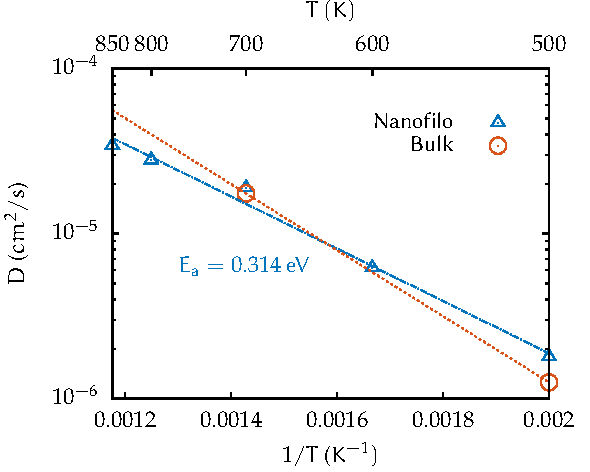
\includegraphics[scale=0.6]{D_vs_T}
  \end{column}


 \end{columns}

\end{frame}


\begin{frame}{Differenza di potenziale chimico}
 Differenza di potenziale chimico $\Delta\mu$ tra cristallo e liquido\\[3pt]
 Formula di {\ev Thompson--Spaepen}
 \[ \Delta\mu = T_m\Delta S_m \frac{(T_m-T)\,2T}{(T_m+T)\,T_m} \]
 \begin{itemize}
 \item $T_m\Delta S_m$ è il calore latente di fusione
 \item $\Delta S_m (\text{bulk})=\num{0.186}\,\si{meV/\text{atomo}}$ da simulazioni MD--NN
 \end{itemize}
 
\end{frame}


\begin{frame}{Velocità di cristallizzazione}{Confronto tra nanofilo e bulk}
 Abbiamo osservato una {\ev diminuzione} della velocità di crescita\\[6pt]
 Supponiamo uguale il valore di $\Delta S_m$ per nanofilo e bulk
 \begin{equation*}
  \begin{split}
   u\ped{N} &= \frac{6D\ped{N}}{\lambda} \left( 1- e^{-\Delta\mu\ped{N}/k_B T} \right) \\[6pt]
   u\ped{B} &= \frac{6D\ped{B}}{\lambda} \left( 1- e^{-\Delta\mu\ped{B}/k_B T} \right)
  \end{split}
 \end{equation*}
 \begin{columns}[b]
  \begin{column}{0.5\textwidth}
   \begin{displaymath}
      \frac{u\ped{N}}{u\ped{B}}(\num{700}\,K) \approx \textcolor{themecolor}{\num{1.61}}
   \end{displaymath}
  \end{column}
  \begin{column}{0.5\textwidth}
   \begin{displaymath}
    \text{Da simulazioni MD} \approx \textcolor{themecolor}{\num{1.78}}
   \end{displaymath}
  \end{column}

 \end{columns}


\end{frame}




%%% BACKUP SLIDES
\appendix

\begin{frame}{Parametro d'ordine}
 \begin{equation*}
  \begin{split}
   \bar{Q}_4(i) &= \frac{1}{N_b(i)}\sum_{j=1}^{N_b(i)}%
  	\frac{\sum_{m=-4}^4 \bar{q}_{4m}(i)\, \bar{q}_{4m}^{\text{*}}(j) }{\left(  \sum_{m=-4}^4 \lvert \bar{q}_{4m}(i)\rvert^2 \right) \left(  \sum_{m=-4}^4 \lvert \bar{q}_{4m}(j)\rvert^2 \right)} \\
  	\bar{q}_{4m}(i) &= \frac{1}{\widehat{N}_{b}(i)} \sum_{k=0}^{\widehat{N}_{b}(i)} q_{4m}(k) \\
  	q_{4m}(i) &= \frac{1}{N_b (i)} \sum_{j=1}^{N_b(i)} Y_{4m}(\bm{r}_{ij})
  \end{split}
 \end{equation*}

\end{frame}


%\begin{frame}{Coefficiente di auto--diffusione}{Calcolo}
% MSD e fit lineare.
%\end{frame}

\begin{frame}{Cristallizzazione}{Confronto tra bulk e nanofilo}
\begin{center}
 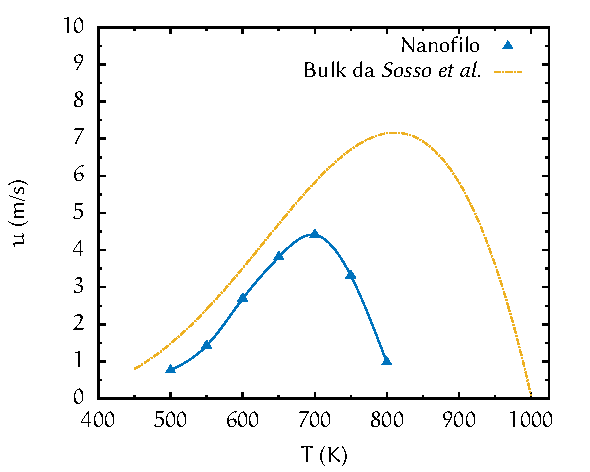
\includegraphics[scale=0.7]{u_vs_T_withSosso}\\[0.2cm]
 {\cit{[Sosso et al., J. Phys. Chem. Lett. 4, 4241 (2013)]}}
\end{center}
\end{frame}





\end{document}


